%!TeX spellcheck = sl_SI
% vim: set spell spelllang=sl:
% za preverjanje črkovanja, če se uporablja Texstudio ali vim
\documentclass[12pt,a4paper,twoside]{article}
\usepackage[utf8]{inputenc}  % pravilno razpoznavanje unicode znakov

% NASLEDNJE UKAZE USTREZNO POPRAVI
\newcommand{\program}{Matematika} % ime studijskega programa
\newcommand{\imeavtorja}{Miha Avsec} % ime avtorja
\newcommand{\imementorja}{doc.~dr.~Anita Buckley} % akademski naziv in ime mentorja, uporabi poln naziv, prof.~dr.~, doc.~dr., ali izr.~prof.~dr.
\newcommand{\imesomentorja}{pred.~mag.~Matjaž Praprotnik} % akademski naziv in ime somentorja, če ga imate
\newcommand{\naslovdela}{Kubične krivulje v kriptografiji}
\newcommand{\letnica}{2019} % letnica magistriranja
\newcommand{\opis}{??.}  % Opis dela v eni povedi. Ne sme vsebovati matematičnih simbolov v $ $.
\newcommand{\kljucnebesede}{kubična krivulja \sep kriptografija \sep ...} % ključne besede, ločene z \sep, da se PDF metapodatki prav procesirajo
\newcommand{\keywords}{cubic curve \sep cryptography} % ključne besede v angleščini
\newcommand{\organization}{Univerza v Ljubljani, Fakulteta za matematiko in fiziko} % fakulteta
\newcommand{\literatura}{literatura}  % pot do datoteke z literaturo (brez .bib končnice)
\newcommand{\sep}{, }  % separator med ključnimi besedami v besedilu
% KONEC PODATKOV

\usepackage{bibentry}         % za navajanje literature v programu dela s celim imenom
\nobibliography{\literatura}
\newcommand{\plancite}[1]{\item[\cite{#1}] \bibentry{#1}} % citiranje v programu dela

\usepackage{filecontents}  % za pisanje datoteke s PDF metapodatki
\usepackage{silence} \WarningFilter{latex}{Overwriting file}  % odstrani annoying warning o obstoju datoteke
% datoteka s PDF metapodatki, zgenerira se kot magisterij.xmpdata
\begin{filecontents*}{\jobname.xmpdata}
  \Title{\naslovdela}
  \Author{\imeavtorja}
  \Keywords{\kljucnebesede}
  \Subject{\opis}
  \Org{\organization}
\end{filecontents*}

\usepackage[a-1b]{pdfx}  % zgenerira PDF v tem PDF/A-1b formatu, kot zahteva knjižnica
\hypersetup{bookmarksopen, bookmarksdepth=3, colorlinks=true,
  linkcolor=black, anchorcolor=black, citecolor=black, filecolor=black,
  menucolor=black, runcolor=black, urlcolor=black, pdfencoding=auto,
  breaklinks=true, psdextra}

\usepackage[slovene]{babel}  % slovenščina
\usepackage[T1]{fontenc}     % naprednejše kodiranje fonta
\usepackage{amsmath,amssymb,amsfonts,amsthm} % matematični paketi
\usepackage[]{color} % barve
\usepackage{graphicx}     % za slike
\usepackage{emptypage}    % prazne strani so neoštevilčene, ampak so štete
\usepackage{units}        % fizikalne enote kot \unit[12]{kg} z polovico nedeljivega presledka, glej primer v kodi
\usepackage{makeidx}      % za stvarno kazalo, lahko zakomentiraš, če ne rabiš
\makeindex                % za stvarno kazalo, lahko zakomentiraš, če ne rabiš
% oblika strani
\usepackage[
  top=3cm,
  bottom=3cm,
  inner=3.5cm,      % margini za dvostransko tiskanje
  outer=2.5cm,
  footskip=40pt     % pozicija številke strani
]{geometry}

% VEČ ZANIMIVIH PAKETOV
% \usepackage{array}      % več možnosti za tabele
% \usepackage[list=true,listformat=simple]{subcaption}  % več kot ena slika na figure, omogoči slika 1a, slika 1b
% \usepackage[all]{xy}    % diagrami
% \usepackage{doi}        % za clickable DOI entrye v bibliografiji
% \usepackage{enumerate}     % več možnosti za sezname

% Za barvanje source kode
% \usepackage{minted}
% \renewcommand\listingscaption{Program}

% Za pisanje psevdokode
% \usepackage{algpseudocode}  % za psevdokodo
\usepackage{algorithm}
\floatname{algorithm}{Algoritem}
\renewcommand{\listalgorithmname}{Kazalo algoritmov}

% DRUGI TVOJI PAKETI:
% tukaj
\usepackage{algorithmicx}
\usepackage{algpseudocode}
\usepackage{listings}


\setlength{\overfullrule}{50pt} % označi predlogo vrstico
\pagestyle{plain}               % samo številka strani na dnu, nobene glave / noge

% ukazi za matematična okolja
\theoremstyle{definition} % tekst napisan pokončno
\newtheorem{definicija}{Definicija}[section]
\newtheorem{primer}[definicija]{Primer}
\newtheorem{opomba}[definicija]{Opomba}
\newtheorem{aksiom}{Aksiom}

\theoremstyle{plain} % tekst napisan poševno
\newtheorem{lema}[definicija]{Lema}
\newtheorem{izrek}[definicija]{Izrek}
\newtheorem{trditev}[definicija]{Trditev}
\newtheorem{posledica}[definicija]{Posledica}

\numberwithin{equation}{section}  % števec za enačbe zgleda kot (2.7) in se resetira v vsakem poglavju

% Matematični ukazi
\newcommand{\R}{\mathbb R}
\newcommand{\N}{\mathbb N}
\newcommand{\Z}{\mathbb Z}
\renewcommand{\C}{\mathbb C}
\newcommand{\Q}{\mathbb Q}

\newcommand{\F}{\mathbb F}
\newcommand{\Fq}[1]{{\mathbb{F}_{#1}}}
\newcommand{\PP}{\mathbb P}
\newcommand{\E}[1]{E({#1})}
\newcommand{\MOD}[1]{\ \text{(mod }{#1}\text{)}}
\newcommand{\DIV}[1]{\ \text{Div(}{#1}\text{)}}
% \DeclareMathOperator{\tr}{tr}  % morda potrebuješ operator za sled ali kaj drugega?

% bold matematika znotraj \textbf{ }, tudi v naslovih, kot \omega spodaj
\makeatletter \g@addto@macro\bfseries{\boldmath} \makeatother

% Poimenuj kazalo slik kot ``Kazalo slik'' in ne ``Slike''
\addto\captionsslovene{
  \renewcommand{\listfigurename}{Kazalo slik}%
}

% če želiš, da se poglavja začnejo na lihih straneh zgoraj
% \let\oldsection\section
% \def\section{\cleardoublepage\oldsection}

%%%%%%%%%%%%%%%%%%%%%%%%%%%%%%%%%%%%%%%%%%
%%%%%%           DOCUMENT           %%%%%%
%%%%%%%%%%%%%%%%%%%%%%%%%%%%%%%%%%%%%%%%%%

\begin{document}

\pagenumbering{roman} % začnemo z rimskimi številkami
\thispagestyle{empty} % ampak na prvi strani ni številke

\noindent{\large
UNIVERZA V LJUBLJANI\\[1mm]
FAKULTETA ZA MATEMATIKO IN FIZIKO\\[5mm]
\program\ -- 2.~stopnja}
% ustrezno dopolni za IŠRM
\vfill

\begin{center}
  \large
  \imeavtorja\\[3mm]
  \Large
  \textbf{\MakeUppercase{\naslovdela}}\\[10mm]
  \large
  Magistrsko delo \\[1cm]
  Mentor: \imementorja \\[2mm] % ustrezno popravi spol
   Somentor: \imesomentorja   % dodaj, če potrebno
\end{center}
\vfill

\noindent{\large Ljubljana, \letnica}

\cleardoublepage

%% IZJAVA O AVTORSTVU
%\pdfbookmark[1]{Izjava o avtorstvu}{izjava} % bookmark v PDF, \pdfbookmark[nivo]{text}{label}
%
%% izjava: po potrebi spremeni v žensko obliko
%\setlength\topsep{0pt}
%\setlength\parskip{0pt}
%\begin{center}
%  \textbf{Univerza v Ljubljani} \\
%  \textbf{Fakulteta za matematiko in fiziko}
%
%  \vfill
%
%  \underline{Izjava o avtorstvu, istovetnosti tiskane in elektronske verzije magistrskega dela in} \\
%  \underline{objavi osebnih podatkov študenta}
%
%  \vfill
%
%  \setlength\topsep{0pt}
%  \setlength\parskip{0pt}
%  \begin{flushleft}
%    Spodaj podpisani študent \imeavtorja{} avtor magistrskega dela (v nadaljevanju: pisnega
%    zaključnega dela študija) z naslovom:
%  \end{flushleft}
%
%  \vfill
%
%  \textbf{\naslovdela}
%
%  \vfill
%
%  IZJAVLJAM
%\end{center}
%
%\begin{enumerate}[1. ]
%  \item \emph{Obkrožite eno od variant a) ali b)}
%  \begin{enumerate}[a)]
%    \item da sem pisno zaključno delo študija izdelal samostojno;
%    \item da je pisno zaključno delo študija rezultat lastnega dela več kandidatov in izpolnjuje
%      pogoje, ki jih Statut UL določa za skupna zaključna dela študija ter je v zahtevanem deležu
%      rezultat mojega samostojnega dela;
%  \end{enumerate}
%  pod mentorstvom IZPOLNI. % dopiši \imementorja v rodilniku
%%   \\ in somentorstvom IZPOLNI. % dopiši \imesomentorja v rodilniku
%  \item da je tiskana oblika pisnega zaključnega dela študija istovetna elektronski obliki
%    pisnega zaključnega dela študija;
%  \item da sem pridobil vsa potrebna dovoljenja za uporabo podatkov in avtorskih del v pisnem
%    zaključnem delu študija in jih v pisnem zaključnem delu študija jasno označil;
%  \item da sem pri pripravi pisnega zaključnega dela študija ravnal v skladu z etičnimi načeli in,
%    kjer je to potrebno, za raziskavo pridobil soglasje etične komisije;
%  \item da soglašam, da se elektronska oblika pisnega zaključnega dela študija uporabi za preverjanje
%    podobnosti vsebine z drugimi deli s programsko  opremo za preverjanje podobnosti
%    vsebine, ki je povezana s študijskim informacijskim sistemom fakultete;
%  \item da na UL neodplačno, neizključno, prostorsko in časovno neomejeno prenašam pravico shranitve
%    avtorskega dela v elektronski obliki, pravico reproduciranja ter pravico dajanja pisnega
%    zaključnega dela študija na voljo javnosti na svetovnem spletu preko Repozitorija UL;
%  \item da dovoljujem objavo svojih osebnih podatkov, ki so navedeni v pisnem zaključnem delu študija
%    in tej izjavi, skupaj z objavo pisnega zaključnega dela študija.
%\end{enumerate}
%
%\vfill
%
%\noindent
%Kraj:  \hfill   Podpis študenta: \phantom{prostor za podpis}
%
%\vfill
%
%\noindent
%Datum:
%
%\cleardoublepage
%% END IZJAVA O AVTORSTVU

% zahvala
\pdfbookmark[1]{Zahvala}{zahvala} %
\section*{Zahvala}
Neobvezno.
Zahvaljujem se \dots
% end zahvala -- izbriši vse med zahvala in end zahvala, če je ne rabiš

\cleardoublepage

\pdfbookmark[1]{\contentsname}{kazalo-vsebine}
\tableofcontents

% list of figures
% \cleardoublepage
% \pdfbookmark[1]{\listfigurename}{kazalo-slik}
% \listoffigures
% end list of figures

\cleardoublepage

\section*{Program dela}
\addcontentsline{toc}{section}{Program dela} % dodajmo v kazalo
Mentor naj napiše program dela skupaj z osnovno literaturo. Na literaturo se
lahko sklicuje kot~\cite{lebedev2009introduction}, \cite{gurtin1982introduction},
\cite{zienkiewicz2000finite}, \cite{STtemplate}.

\section*{Osnovna literatura}
Literatura mora biti tukaj posebej samostojno navedena (po pomembnosti) in ne
le citirana. V tem razdelku literature ne oštevilčimo po svoje, ampak uporabljamo
okolje itemize in ukaz plancite, saj je celotna literatura oštevilčena na koncu.
\begin{itemize}
  \plancite{lebedev2009introduction}
  \plancite{gurtin1982introduction}
  \plancite{zienkiewicz2000finite}
  \plancite{STtemplate}
\end{itemize}

\vspace{2cm}
\hspace*{\fill} Podpis mentorja: \phantom{prostor za podpis}

% \vspace{2cm}
% \hspace*{\fill} Podpis somentorja: \phantom{prostor za podpis}

\cleardoublepage
\pdfbookmark[1]{Povzetek}{abstract}

\begin{center}
\textbf{\naslovdela} \\[3mm]
\textsc{Povzetek} \\[2mm]
\end{center}
Tukaj napišemo povzetek vsebine. Sem sodi razlaga vsebine in ne opis tega, kako je delo
organizirano.

\vfill
\begin{center}
\textbf{English translation of the title} \\[3mm] % prevod slovenskega naslova dela
\textsc{Abstract}\\[2mm]
\end{center}

An abstract of the work is written here. This includes a short description of
the content and not the structure of your work.

\vfill\noindent
\textbf{Math.~Subj.~Class.~(2010):} oznake kot 74B05, 65N99, na voljo so na naslovu
\url{http://www.ams.org/msc/msc2010.html?t=65Mxx} \\[1mm]
\textbf{Ključne besede:} \kljucnebesede \\[1mm]
\textbf{Keywords:} \keywords

\cleardoublepage

\setcounter{page}{1}    % od sedaj naprej začni zopet z 1
\pagenumbering{arabic}  % in z arabskimi številkami



%%%%%%%%%%%%%%%%%%%%%%%%%%%%%%%%%%%%%%%%%%%%%%%%%%%%%%%%%%%%%%%%%%%%%%%%%%%%%%%%%%%%%%
%UVOD
%%%%%%%%%%%%%%%%%%%%%%%%%%%%%%%%%%%%%%%%%%%%%%%%%%%%%%%%%%%%%%%%%%%%%%%%%%%%%%%%%%%%%%
\section{Uvod}
Kubične krivulje se v kriptografiji uporabljajo, ker zagotavljajo isto varnost, kot drugi klasični kriptosistemi, pri tem pa potrebujejo manjšo velikost ključa. Ocenjuje se, da je $2048$ bitni ključ v RSA algoritmu enako varen kot $224$ bitni ključ nad kubičnimi krivuljami. Krajši kluči predstavljajo veliko prednost v okoljih s slabšo procesorsko močjo in/ali omejenim pomnilnikom. Primer take uporabe predstavljajo pametne kartice. Uporaba kubičnih krivulj v namene kriptografije je prvi predlagal Victor S. Miller leta 1985, a so le te v širšo rabo vstopile še le okoli leta 2004.


%%%%%%%%%%%%%%%%%%%%%%%%%%%%%%%%%%%%%%%%%%%%%%%%%%%%%%%%%%%%%%%%%%%%%%%%%%%%%%%%%%%%%%
%KUBIČNE KRIVULJE
%%%%%%%%%%%%%%%%%%%%%%%%%%%%%%%%%%%%%%%%%%%%%%%%%%%%%%%%%%%%%%%%%%%%%%%%%%%%%%%%%%%%%%
\section{Kubične krivulje}


KOPIRANO IZ DIPLOME ALI JE OK????

\subsection{Točke na krivulji}

\begin{definicija}~

\emph{Projektivna ravnina} $\mathbb{P}^2$ nad poljem $\F$ je kvocientni prostor $\F^3-\{0\}/\! \!\sim$, kjer je ekvivalenčna relacija podana z $(a,b,c)\sim(\alpha a,\alpha b,\alpha c)$ za vsak $\alpha \in \F \setminus \{0\}$. Točke v $\mathbb{P}^2$ so torej podane s homogenimi koordinatami $[a,b,c] = [\alpha a,\alpha b,\alpha c]$ za vse $\alpha \neq 0$.
\end{definicija} 

Točko projektivne ravnine si lahko predstavljamo kot premico skozi izhodišče, kot prikazuje slika \ref{fig:ravnina}.


\begin{figure}[h]
  \centering
  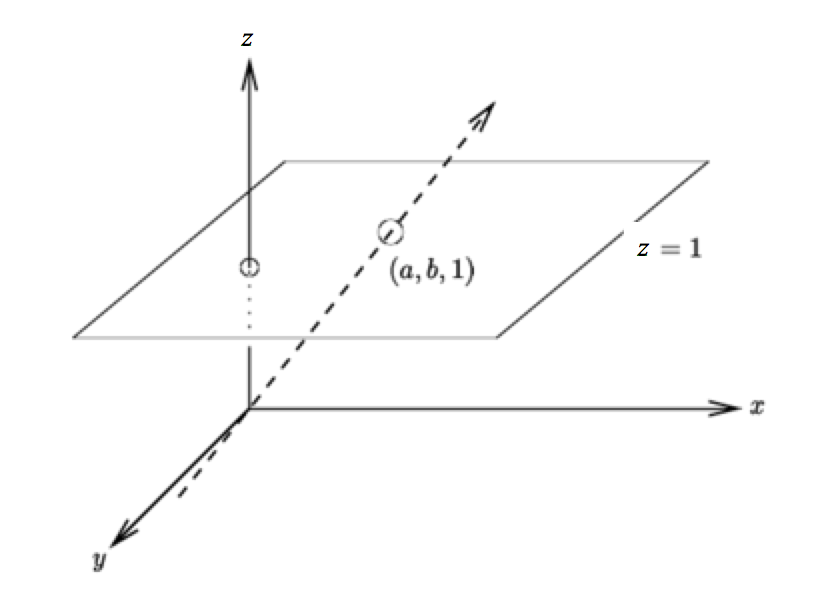
\includegraphics[width=0.6\textwidth]{images/ravnina.png}
% \caption[caption za v kazalo]{Dolg caption pod sliko}
  \caption[Primer točke v projektivni ravnini.]{Točka [a,b,1] v projektivni ravnini.}
  \label{fig:ravnina}
\end{figure}


\begin{definicija}~

Polinom $P$ je \emph{homogen} stopnje $d$, če velja $P(\lambda x,\lambda y, \lambda z) = \lambda ^d P(x,y,z)$ za vse $\lambda \in \F$.
\end{definicija}

\begin{definicija}~

\emph{Algebraična krivulja}, podana s homogenim polinomom $P$, je množica točk 
$$\mathcal{C}_P= \{ A \in \mathbb{P}^2, P(A) = 0 \}.$$
\end{definicija}

\emph{Kubična krivulja} je algebraična krivulja, podana s homogenim polinomom stopnje 3. V splošnem je torej oblike
\begin{align}
&{} a_{300}x^3+a_{210}x^2y+a_{201}x^2z+a_{120}xy^2+a_{102}xz^2+ \nonumber \\
&{}+a_{012}yz^2+a_{030}y^3+a_{003}z^3+a_{111}xyz+a_{021}y^2z = 0, \nonumber
\end{align}
kjer so $a_{ijk} \in \F$.
Ta zapis vsebuje $10$ koeficientov, vendar se v gladkih primerih lahko polinom poenostavi.
\begin{definicija}~\\
Algebraična krivulja je \emph{gladka}, če nima nobenih samopresečišč ali singularnosti.
\end{definicija}

\begin{izrek}[\protect{\cite{gibson}, Izrek 15.2}]~

Gladko kubično krivuljo nad algebraično zaprtim poljem lahko zapišemo v Weierstrassovi obliki
$$y^2z = x^3 + axz^2 + bz^3.$$
\end{izrek}

\begin{primer}~

Polinom $P(x,y,z) = z^2y-x^3$ je homogen polinom stopnje $3$. Rešitve enačbe $z^2y-x^3 = 0$ pa podajajo točke na kubični krivulji.
\\


\begin{figure}[ht]
  \centering
\begin{minipage}{.5\textwidth}
  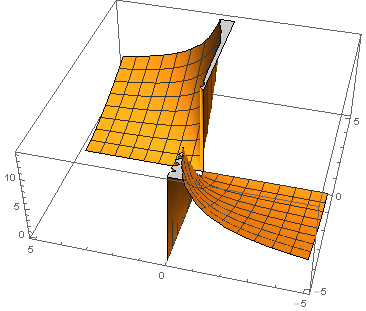
\includegraphics[width=0.8\textwidth]{images/krivulja.png}
  \caption[Primer algebraične krivulje.]{Algebraična krivulja, podana s polinomom $z^2y-x^3$.}
  \label{fig:krivulja}
\end{minipage}%
\begin{minipage}{.5\textwidth}
\centering
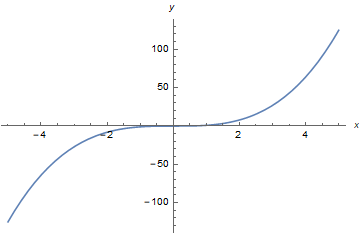
\includegraphics[scale=0.5]{images/projektivnaz.png}
\caption[Presek algebraične krivulje z ravnino $z=1$.]{Presek algebraične krivulje z ravnino $z=1$.}
\label{fig:projektivnaz}
\end{minipage}
\end{figure}


\begin{figure}[ht]
\centering
\begin{minipage}{.5\textwidth}
\centering
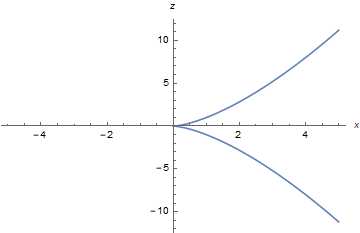
\includegraphics[scale=0.5]{images/projektivnay.png}
\caption[Presek algebraične krivulje z ravnino $y=1$.]{Presek algebraične krivulje z ravnino $y=1$.}
\label{fig:projektivnay}
\end{minipage}%
\begin{minipage}{.5\textwidth}
\centering
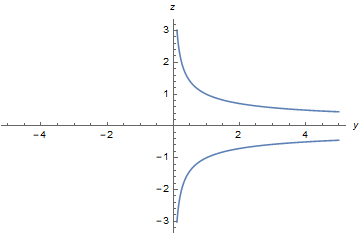
\includegraphics[scale=0.5]{images/projektivnax.png}
\caption[Presek algebraične krivulje z ravnino $x=1$.]{Presek algebraične krivulje z ravnino $x=1$.}
\label{fig:projektivnax}
\end{minipage}
\end{figure}


Na zgornjih slikah lahko vidimo, kako krivuljo predstavimo v projektivni ravnini, ter njene preseke z različnimi afinimi ravninami.

\end{primer}



V nadaljevanju nas bodo zanimale predvsem gladke kubične krivulje v polju $\mathbb{Z}/n\mathbb{Z}$.

\begin{definicija}~
Za dani števili $a$, $b \in \mathbb{Z}/n\mathbb{Z}$ je \emph{kubična krivulja} nad poljem $\mathbb{Z}/n\mathbb{Z}$ množica točk
$$E_{(a,b)}(\mathbb{Z}/n\mathbb{Z}) =\left\{ [x,y,z] \in \PP^2(\mathbb{Z}/n\mathbb{Z}): y^2z=x^3+axz^2+bz^3 \right\} .$$
Drugače povedano, afina kubična krivulja je množica rešitev enačbe
$$y^2=x^3+ax+b.$$
Pri čemer upoštevamo zvezo med afinimi in projektivnimi koordinatami točk:
$$(x,y)\in (\Z/n\Z)^2 \Leftrightarrow [x,y,1]\in \PP^2(\Z/n\Z).$$

\end{definicija}
\newpage
\subsection{Struktura grupe na kubičnih krivuljah}
Za definicijo grupe na kubičnih krivuljah uvedimo najprej pomožno operacijo

$$\ast : \mathcal{C}_P \times \mathcal{C}_P \rightarrow \mathcal{C}_P,$$
tako da za poljubni točki $A$, $B$ na krivulji velja:

\[ A \ast B =
\begin{cases}
A & \quad \text{če je } A=B \ \text{prevoj},\\
C & \quad \text{če je } \overline{AB} \cap \mathcal{C}_P = \left\{ A,B,C \right\},\\
A & \quad \text{če je } \overline{AB} \ \text{tangenta v } A,\ \text{ter} \ A \neq B,\\
B & \quad \text{če je } \overline{AB} \ \text{tangenta v } B,\ \text{ter} \ A \neq B,\\
C &\quad \text{če je } A=B \ \{\text{in tangenta v A}\} \cap \mathcal{C}_P = \left\{ A,C \right\}.\\
\end{cases}
\]
Intuitivno operacija $\ast$ vrne tretjo točko v preseku premice skozi $A$ in $B$ in $\mathcal{C}_P$. Poglejmo si še nekaj lastnosti operacije $\ast$. Dokaze sledečih trditev najdemo v \cite[Poglavje 17.3]{gibson}.

\begin{trditev}~

\label{last zvezda}
Operacija $\ast$ ima naslednje lastnosti:

\begin{itemize}
\item komutativnost: $ A \ast B = B \ast A$,
\item absorpcija: $(A \ast B ) \ast A = B$ ,
\item $((A \ast B) \ast C ) \ast D = A \ast ((B \ast D)\ast C)$.
\end{itemize}
\end{trditev}

\begin{izrek}~

Kubična krivulja ($\mathcal{C}_P$,$+$) je Abelova grupa za operacijo

\begin{table}[ht]
\centering
\begin{tabular}{llll}
$+:$ & $\mathcal{C}_P \times \mathcal{C}_P$ & $\rightarrow$ & $\mathcal{C}_P$ \\
& $(A,B)$ & $\rightarrow$ & $(A\ast B)\ast O$ ,
\end{tabular}
\end{table}
kjer je $O$ poljubna izbrana točka na krivulji $ \mathcal{C}_P$.
\end{izrek}

\begin{proof}~

S pomočjo trditve \ref{last zvezda} dokažimo, da je ($\mathcal{C}_P$,$+$) res Abelova grupa.

\begin{itemize}
\item Operacija $+$ je komutativna:
$$A+B = (A \ast B ) \ast O = (B \ast A) \ast O = B+A.$$
\item Točka O je nevtralni element:
$$A+O=(A \ast O) \ast O = A.$$
\item Nasprotni element A definiramo kot $-A = A \ast (O \ast O )$ in preverimo:
\begin{align}
A + (-A) &{} = (A \ast (A \ast (O \ast O))) \ast O \nonumber \\
&{} = (O \ast O) \ast O \nonumber \\
&{} = O, \nonumber
\end{align}
kjer smo uporabili absorbcijo.
\item Asociativnost $(A + B) + C = A + (B + C)$ dokažemo z računom:
\begin{align}
(A + B) + C &{} = ((A + B) \ast C) \ast O \nonumber \\
&{} = (((A \ast B) \ast O) \ast C) \ast O \nonumber \\
&{} = (A \ast ((B \ast C) \ast O)) \ast O \nonumber \\
&{} = (A \ast (B + C)) \ast O = A + (B + C). \nonumber \qedhere
\end{align}
\end{itemize}
\end{proof}

Ta definicija operacije nudi eleganten opis strukture grupe, za numerično računanje pa ni primerna. Možno pa je izpeljati formule, s katerimi lahko eksplicitno
izračunamo vsoto dveh točk, v kolikor imamo kubično krivuljo v Weierstrassvi obliki.

\begin{lema}[Seštevanje točk na Weierstrassovi kubični krivulji]~

\label{sestevanje}
Naj bo $\mathcal{C}_P$ afina krivulja v Weierstrassovi obliki $y^2 = x^3 + \alpha x^2 + \beta x + \gamma$, ter $O$ prevoj v neskončnosti. Če sta $A_1 = (a_1,b_1)$ in $A_2 = (a_2,b_2)$ točki na afinem delu $\mathcal{C}_P$, potem za $A_3 = A_1 + A_2 = (a_3,b_3)$ velja

\begin{align}
&{} a_3 = \lambda ^2 - \alpha - a_1 - a_2 \nonumber \\
&{} b_3 = -\lambda a_3 - \mu, \nonumber
\end{align}
kjer sta 

\[ \lambda =
\begin{cases}
\frac{b_1 - b_2}{a_1 - a_2} & \quad \text{če } a_1 \neq a_2 ,\\
\frac{3a_1^2+ 2 \alpha a_1 + \beta}{2b_1} & \quad \text{sicer} ,\\
\end{cases}
\]

ter $\mu = b_1 - \lambda a_1$.

\end{lema}


\begin{opomba}
Če krivuljo $\mathcal{C}_P$ predstavimo v projektivni ravnini, torej s homogenim polinomom $yz^2=x^3+\alpha x^2z+\beta xz^2+ \gamma yz^2$ je prevoj $O=[0,1,0].$
\end{opomba}

\begin{primer}~

Na spodnji sliki je v afini ravnini $y=1$ prikazano kako grafično seštevamo točke na Weierstrassovi kubiki $yz^2-x(x-y)(x+y)=0$. Sešteti želimo točki $A =(-1,0)$ in $B=(2,\sqrt{6}) $.
\\


\begin{figure}[h]
  \centering
  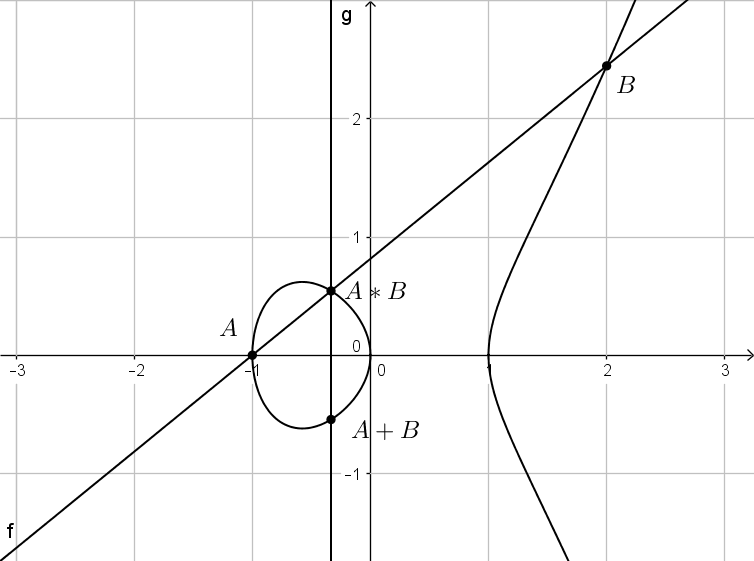
\includegraphics[width=0.8\textwidth]{images/adicija.png}
  \caption[Grafično seštevanje.]{Grafično seštevanje točk na kubični krivulji.}
  \label{fig:adicija}
\end{figure}

\end{primer}



\begin{primer}~

Seštejmo točki $A =(-1,0),B=(2,\sqrt{6}) $ na Weierstrassovi kubični krivulji $yz^2-x(x-y)(x+y)=0$ v preseku s projektivno ravnino $y=1$ še računsko z uporabo zgornje leme \ref{sestevanje}.
Prepišimo našo krivuljo najprej v afino obliko iz leme \ref{sestevanje}. Ker smo v ravnini $y=1$, najprej zamenjajmo vlogi $y$ in $z$.

$$z^2-x(x-1)(x+1) = 0 $$ 
Dobimo $z^2 = x^3-x,$
torej je $\alpha = 0$, $\beta = -1$ in $\gamma=0$. Izračunajmo sedaj $\lambda$ in $\mu$, pri čemer upoštevamo prvi predpis, saj sta x-koordinati točk različni:
$$\lambda = \frac{-\sqrt{6}}{-1-2} = \frac{\sqrt{6}}{3},$$

$$\mu = 0 - \frac{\sqrt{6}}{3} (-1) = \frac{\sqrt{6}}{3}.$$

Koordinati vsote $A+B=(x,y)$ sta torej enaki

$$x = \frac{6}{9} - 0+1-2=-\frac{1}{3}$$

in

$$z = -\frac{\sqrt{6}}{3}(-\frac{1}{3})-\frac{\sqrt{6}}{3}=-\frac{2\sqrt{6}}{9} \doteq -0.5443.$$

Iskana točka $A+B \in \PP^2$ je torej enaka $[-\frac{1}{3},1,-\frac{2\sqrt{6}}{9}]$. Dobljeni rezultat se ujema s točko, ki smo jo dobili z grafičnim seštevanjem.

\end{primer}

%%%%%%%%%%%%%%%%%%%%%%%%%%%%%%%%%%%%%%%%%%%%%%%%%%%%%%%%%%%%%%%%%%%%%%%%%%%%%%%%%%%%%%
%DIEFFIE-HELLMAN
%%%%%%%%%%%%%%%%%%%%%%%%%%%%%%%%%%%%%%%%%%%%%%%%%%%%%%%%%%%%%%%%%%%%%%%%%%%%%%%%%%%%%%

\section{Diffie-Hellmanova izmenjava ključev nad gladkimi kubičnimi krivuljami}

Diffe-Hellmanova izmenjava ključev je postopek, pri katerem se dve osebi npr.\  Alenka in Boris dogovorita za skrivni ključ na takšen način, da tudi v primeru ko njun pogovor posluša tretji nepovabljeni gost npr.\  Ciril le ta iz pogovora ne more rekonstruirati ključa za katerega sta se tekom pogovora dogovorila Alenka in Boris. 
\begin{algorithm}[H]
\caption[Diffe-Hellman]{Diffie-Hellmanova izmenjava ključev.}
\label{alg:diffie-hellman}

\begin{enumerate}

\item Alenka in Boris se dogovorita za elitpično krivuljo $E$ nad končnim obsegom $\F{q}$, ter za točko $P \in \E{\Fq{q}}$.
\item Alenka se odloči za skrivno število $a \in \N$, in izračuna $P_a = aP$, ter to pošlje Borisu.
\item Boris se odloči za skrivno število $b \in \N$, in izračuna $P_b = bP$, ter to pošlje Alenki.
\item Alenka izračuna $aP_b=abP$.
\item Boris izračuna $bP_a=baP$.

\end{enumerate}
\end{algorithm}

Kot sam ključ bi lahko na koncu Alenka in Boris uporabila npr.\  zadnjih $256$ bitov x-koordinate točke $abP$. Tu se zanašamo na to, da je iz $E, \F{q},P, P_a, P_b$ težko izračunati $baP$. Zelo veliko pa je tu odvisno od same izbire krivulje E.

To nas privede do t.\ i.\ problema diskretnega logaritma.


\begin{definicija}~
Naj bosta $a, b \in \N$, ter naj bo p praštevilo. Iščemo število k tako, da bo
$$a^k \equiv b\ (\text{mod} \ p).$$
\end{definicija}

\begin{trditev}~
Če lahko rešimo problem diskretnega logaritma, potem smo rešili tudi problem Diffie-Hellmanove izmenjave ključev. Povedano drugače velja
$$\text{DL} \Rightarrow DH.$$
\end{trditev}

\begin{proof}
Problem Diffie-Hellmanove izmenjave ključev lahko enostavno prevedemo na problem diskretnega logaritma na sledeč način:

\begin{itemize}
\item Vzemi $aP$ in izračunaj $a$ tako, da rešiš problem diskretnega logaritma.
\item Izračunaj $a(bP)$.
\end{itemize}

\end{proof}

\subsection{Index Calculus}
\label{IndexCalc}

Naj bo $p$ praštevilo in naj bo $g$ generator ciklične grupe $\F^{\times}_{p}$. Naj $L(h)$ označuje vrednost, za katero velja
$$g^{L(h)} \equiv h \ (\text{mod} \ p).$$
Iz definicije $L(h)$ sledi, da velja $$L(h_1h_2) = L(h_1)+L(h_2) \ (\text{mod} \ p).$$
Idejo napada na problem diskretnega logaritma v taki grupi najlažje vidimo na primeru.

\begin{primer}
Naj bo $p = 1217$ in $g= 3$. Rešiti hočemo $3^k \equiv 37 \mod 1217$. Izberimo si bazo praštevil $\{ 2,3,5,7,11,13 \}$. Pri tem upoštevamo, da bo večja baza pomenila več računanja a hkrati lažjo pot do odgovora. Išemo $x$-e  tako, da bo
$$3^x \equiv \pm \text{produktu praštevil iz baze} \mod 1217.$$

Ob iskanju takih $x$ najdemo naslednje enakosti:
\begin{align}
3^1 &\equiv 3 \MOD{1217} \nonumber \\ 
3^{24}  &\equiv -2^2\cdot 7\cdot 13 \MOD{1217} \nonumber \\
3^{25}  &\equiv 5^3 \MOD{1217} \nonumber \\
3^{30}  &\equiv -2 \cdot 5^2 \MOD{1217} \nonumber \\
3^{54}  &\equiv -5\cdot 11 \MOD{1217} \nonumber \\
3^{87}  &\equiv 13 \MOD{1217} \nonumber
\end{align}
Z večjo bazo bi v tem primeru lažje našli take enačbe, a bi jih hkrati potrebovali več.
Z uporabo malega Fermatovega izreka, velja
$$3^{1216} \equiv 1 \equiv (-1)^2 \mod 1217, $$
od koder sledi $L(-1) \equiv 608 \mod 1216$.
Če enačbe sedaj zapišemo z uporabo $L(h)$, dobimo
\begin{align}
1 &\equiv L(3) \MOD{1216} \nonumber \\ 
24&\equiv 608 + 2L(2) + L(7) +L(13) \MOD{1216} \nonumber \\
25 &\equiv 3L(5) \MOD{1216} \nonumber \\
30 &\equiv 608+L(2)+2L(5) \MOD{1216} \nonumber \\
54 &\equiv 608+L(5)+L(11) \MOD{1216} \nonumber \\
87  &\equiv L(13) \MOD{1216}  \nonumber
\end{align}

Od tod bobimo $L(2) = 216, L(11)=1059,L(7) = 113,L(5) = 819,L(13) = 87,L(3)=1$.
Sedaj poračunamo za različne $j$ vrednost $3^j*37$, dokler ne dobimo $3^j*37 \equiv \text{produktu elementov iz baze}$.
Pri vrednosti $j=16$ dobimo
$$3^{16}\cdot 37 \equiv 2^3\cdot 7 \cdot 11 \MOD{1217}.$$
Iščemo $L(37)$, iz definicije $L$ pa velja
$$3^{L(37)} \equiv 37 \MOD{1217} \equiv 2^3\cdot 7 \cdot 11 \cdot 3^{-16}\MOD{1217}.$$
Če sedaj namesto baze vstavimo primerne $L$ dobimo
$$3^{L(37)} \equiv 3^{3L(2)}\cdot 3^{L(7)} \cdot 3^{L(11)} \cdot 3^{-16L(3)}\MOD{1217}.$$
$L(37)$ lahko sedaj zapišemo kot
$$L(37) \equiv 3L(2) +L(7)+L(11) - 16L(3) \MOD{1216} \equiv 588 \MOD{1216}.$$

Torej je naš iskani $k=588$.

\end{primer}
\subsection{Index Calculus program}

\lstinputlisting[language=Python]{IndexCalculus.py}
%%%%%%%%%%%%%%%%%%%%%%%%%%%%%%%%%%%%%%%%%%%%%%%%%%%%%%%%%%%%%%%%%%%%%%%%%%%%%%%%%%%%%%
%PARJENJA
%%%%%%%%%%%%%%%%%%%%%%%%%%%%%%%%%%%%%%%%%%%%%%%%%%%%%%%%%%%%%%%%%%%%%%%%%%%%%%%%%%%%%%
\section{Parjenja}

Parjenja imajo pomembno vlogo pri napadih na problem diskretnega logaritma nad gladkimi kubičnimi krivuljami.

\begin{definicija}~
\emph{Eliptična} krivulja je gladka kubična krivulja.
\end{definicija}

\begin{definicija}~
Naj bo $E$ eliptična krivulja nad poljem $K$, ter naj bo $n\in \N$. \emph{Torizjske točke} so množica
$$E[n] = \{ P \in \E{\overline{K}} | nP = \infty \}.$$
\end{definicija}

\begin{izrek}
\label{IzrekTor}
Naj bo $E$ eliptična krivulja nad poljem $K$ in naj bo $n \in \N$. Če karakteristika polja $K$ ne deli $n$, ali je enaka $0$ potem
$$E[n] \cong \mathbb{Z}_n \oplus \mathbb{Z}_n$$

\end{izrek}

\begin{proof}
Se ne vem kako bo napisan
\end{proof}

\begin{definicija}~
Definirajmo \emph{deliteljski polinom} $\gamma_m \in \Z[x,y,A,B]$ kot,


\begin{align}
\gamma_0 &{}= 0  \nonumber \\
\gamma_1 &{}= 1  \nonumber \\
\gamma_2 &{}= 2y  \nonumber \\
\gamma_3 &{}= 3x^4 + 6Ax^2 + 12Bx-A^2 \nonumber \\
\gamma_4 &{}= 4y(x^6+5Ax^4+20Bx^3-5A^2x^2-4ABx-8B^2-A^3) \nonumber \\
\gamma_{2m+1} &{}= \gamma_{m+2}\gamma_{m}^3-\gamma_{m-1}\gamma_{m+1}^3 \text{za } m \geq 2 \nonumber \\
\gamma_{2m} &{}= (2y)^{-1}\gamma_{m}(\gamma_{m+2}\gamma_{m-1}^2-\gamma_{m-2}\gamma_{m+1}^2)\text{za } m \geq 3 \nonumber
\end{align}

\end{definicija}

\begin{lema}

$\gamma_{n}$ je element $\Z[x,y^2,A,B]$, za vse lihe $n$.  Za sode $n$ pa je $\gamma_{n}$ element $2y\Z[x,y^2,A,B]$.

\end{lema}

\begin{proof}
Dokažimo to s pomočjo indukcije. Za $n \leq 4$ lema očitno velja. Obravnavajmo primera, ko je $n=2m$ in  $n=2m+1$ za nek $m\in\N$.
\begin{itemize}
\item{n=2m}
Indukcijska predpostavka je v tem primeru, da lema velja za vse $n<2m$.
Predpostavimo lahko, da je $2m>4$, saj vemo da lema velja za $n\leq 4$, torej velja $m>2$. Potem velja $2m>m+2$, kar pomeni, da vsi polinomi v definiciji $\gamma_{2m}$ zadoščajo indukcijski predpostavki. Če je $m$ sodo število ,potem se $\gamma{m},\gamma{m+2},\gamma{m-2}$ nahajajo v $2y\Z[x,y^2,A,B]$. Od tod pa sledi, da je tudi $\gamma_{2m} \in 2y\Z[x,y^2,A,B]$.
Če je $m$ lih, potem sta $\gamma{m-1},\gamma{m+1} \in 2y\Z[x,y^2,A,B]$. To pa pomeni, da je tudi  $\gamma_{2m} \in 2y\Z[x,y^2,A,B]$.
\item{n=2m+1}
Primer obravnavamo podobno kot $n=2m$.


\end{itemize}


\end{proof}

\begin{definicija}~
Naj bo $K$ polje in naj bo $n \in \N$ tak, da karakteristika $K$ ne deli $n$.
$$\mu_n = \{ x \in \overline{K} | x^n = 1 \}$$
je \emph{grupa n-tih korenov enote} grupe $\overline{K}$.
\end{definicija}

\begin{trditev}
\label{trd-WeilPar}
Naj bo E eliptična krivulja definirana nad poljem $K$, in naj bo $n \in \N$. Predpostavimo, da karakteristika polja $K$ ne deli $n$. Potem obstaja Weilovo parjenje
$$e_n:E[n] \times E[n] \rightarrow \mu_n,$$
za katerega velja:
\begin{itemize}
\item $e_n$ je bilinearna v obeh spremenljivkah
$$e_n(S_1+S_2,T) = e_n(S_1,T)e_n(S_2,T)$$
in
$$e_n(S,T_1+T_2) = e_n(S,T_1)e_n(S,T_2)$$
za vse $S,S_1,S_2,T,T_1,T_2 \in E[n]$.
\item $e_n$ je nedegenerirana v obeh spremenljivkah. To pomeni če je $e_n(S,T) = 1$ za vse $T \in E[n]$ potem $S = \infty$, ter obratno.

\item $e_n(T,T) = 1$ za vse $T \in E[n]$

\item $e_n(T,S) = e_n(S,T)^{-1}$ za vse $S,T \in E[n]$

\item $e_n(\rho S,\rho T) = \rho(e_n(S,T))$ za vse avtomorfizme $\rho$ iz $\bar{K}$, za katere je $\rho$ identiteta na koeficientih $E$.

\item $e_n(\alpha(S),\alpha(T)) = e_n(S,T)^{\text{deg}(\alpha)}$ za vse separabilne endomorfizme $\alpha$ polja $E$.
\end{itemize}

\end{trditev}

\begin{proof}
%%%%%%%%%%%%
%POMEMBNO
%manka utemeljitev da je E[n] \subset E(K) in pa \mu_n \subset E(K)
Naj bo $T \in E[n]$.
Po izreku \ref{izrek 11.2} obstaja funkcija $f$, tako da velja
\begin{equation}
\label{enacba-Weil}
div(f) = n[T]-n[\infty].
\end{equation}
To drži ker je $D = n[T]-n[\infty]$ delitelj za katerega velja $deg(D) = 0$. Prav tako pa velja $sum(D) = \infty$, ker se nahajamo v $E[n]$.
Izberimo sedaj še točko $T' \in E[n^2]$, za katero velja $nT' = T$. Pokazati želimo, da obstaja funkcija $g$, tako da velja
$$div(g) = \sum_{R \in E[n]}([T' + R]- [R]).$$
Preden lahko uporabimo izrek \ref{izrek 11.2} moramo preveriti, da vse potrebne lastnosti držijo. Veljati mora torej $$sum( \sum_{R \in E[n]}([T' + R]- [R])) = \infty$$ in $$deg( \sum_{R \in E[n]}([T' + R]- [R])) = 0.$$
Po izreku \ref{IzrekTor}, se da $E[n]$ zapisati kot $\mathbb{Z}_n \oplus \mathbb{Z}_n$. To pomeni, da $E[n]$ vsebuje $n^2$ različnih točk $R$. Velja torej
$$sum(\sum_{R \in E[n]}([T' + R]- [R])) = \sum_{R \in E[n]} T' +R-R = \sum_{R \in E[n]} T' = n^2T' = nT = \infty.$$
Podobno preverimo, še da velja $deg(\sum_{R \in E[n]}([T' + R]- [R])) = 0.$ Torej po izreku \ref{izrek 11.2} taka funkcija $g$ obstaja.
Označimo z $f \circ n$ funkcijo, ki začne z neko točko jo pomnoži z $n$ in nato na njej uporabi $f$. Točke $P = T' + R$, kjer je $R\in E[n]$ so točke za katere velja $nP=T$. Iz \ref{enacba-Weil}
sledi
%zakaj je to res
%????????????????????????????????????????????????????
$$div(f \circ n) = n(\sum_{R \in E[n]}[T' + R]) - n(\sum_{R \in E[n]}[R]) = div(g^n).$$
Iz definicije delitelja funckije sledi, da je funkcija $f \circ n$ oblike $g^n$ krat neka konstanta. Če za nov $f$ vzamemo ta $f$ pomnožen s primerno konstanto potem lahko predpostavimo, da velja
$$f \circ n = g^n.$$
Naj bo $S \in E[n]$, ter naj bo $P \in \E{\overline{K}}$. Potem velja
$$g(P+S)^n = f(n(P+S)) = f(nP) = g(P)^n.$$
Zaradi tega velja $g(P+S)/g(P) \in \mu_n$.
Tako lahko sedaj definiramo Weilovo parjenje kot
$$e_n(S,T) = \frac{g(P+S)}{g(P)}.$$
Ta definicija je dobra, ker je $g$ zaradi delitelja določen do skalarja natančno, zaradi tega pa je definicija neodvisna od izbire $g$. Prav tako pa je definicija noedvisna od izbire $P$, a je obrazložitev bolj zahtevna in je ne bomo navedli.

Sedaj, ko smo uspeli definirati Weilovo parjenje moramo preveriti, da zanj veljajo lastnosti $1$-$6$.
\begin{enumerate}
\item Ker je definicija neodvisna od izbire točke $P$ lahko uporabimo $P,P+S_1$.
\begin{align}
e_n(S_1,T)e_n(S_2,T) &{}= \frac{g(P+S_1)}{g(P)} \frac{g(P+S_1+S_2)}{g(P+S_1)} \nonumber \\
&{} = \frac{g(P+S_1+S_2)}{g(P)} \nonumber \\
&{} = e_n(S_1+S_2,T). \nonumber
\end{align}
Pokazati moramo še
$$e_n(S,T_1)e_n(S,T_2) = e_n(S,T_1+T_2).$$
Dokaz linearnosti v drugi spremenljivki pa je malce težji kot dokaz za prvo spremenljivko.
Predpostavimo da $T_1,T_2,T_3 \in E[n]$ z lastnostjo $T_1 +T_2 = T_3.$ Označimo z $f_i,g_i$ funkcije ki spdajo k definicijam $e_n(S,T_i)$.
Po izreku \ref{izrek 11.2} obstaja funkcija $h$, za katero velja
$$div(h) = [T_3]-[T_1]-[T_2] + [\infty].$$

Enačba \ref{enacba-Weil} nam da
$$div \left(  \frac{f_3}{f_1f_2}\right) = n div(h) = div(h^n).$$
Zato obstaja konstanta $c \in \overline{K}^{\times}$, tako da velja
$$f_3 = cf_1f_2h^n.$$
Od tod pa sledi
$$g_3 = c^{1/n}(g_1)(g_2)(h \circ n)$$.

To pa nas končno pripelje do
\begin{align}
e_n(S,T_1+T_2) &{}= \frac{g_3(P+S)}{g_3(P)} = \frac{g_1(P+S)}{g_1(P)} \frac{g_2(P+S)}{g_2(P)} \frac{h(n(P+S))}{h(nP)} \nonumber \\
&{} = e_n(S,T_1)e_n(S,T_2). \nonumber
\end{align}

Tu smo upoštevali $nS = \infty$, od koder sledi $h(n(P+S)) = h(nP)$.

\item Predpostavimo, da $T \in E[n]$, tak da velja $e_n(S,T)=1$ za vse $S \in E[n]$. To pomeni, da je $g(P+S) = g(P)$ za vse $P$ in $S \in E[n]$. Po trditvi \ref{manka}%manka%%%%%%%%%%%%%%%%%%%%%%%%%%%%%%%%%%%%%%%%%
obstaja funkcija $h$, tako da velja $g = h \circ n$. Od tod sledi 
$$(h \circ n) ^n = g^n = f \circ n.$$
Ker je množenje z $n$ surjektivno na $E(\overline{K})$, od tod sledi $h^n = f$. %%%%%%%%%%%%%%%%ZAKAJ TO RES
To pa pomeni
$$ndiv(h) = div(f) = n[T]-n[\infty],$$
kar pa pomeni, da je $div(h) = [T] - [\infty]$. Po izreku \ref{izrek 11.2} pa od tod sledi $T = \infty$. S tem smo, dokazali eno polovico točke $2$, druga polovica pa avtomatično sledi iz tega ter uporabe točke $4$.

\item Označimo z $\tau_{jT}$ točko $jT$. V tem primeru $f \circ \tau_{jT}$ označuje funkcijo \newline $P \mapsto f(P+jT)$. Delitelj te funkcije je torej $n[T-jT]-n[-jT]$. Zaradi tega velja

\begin{align}
&{}div(\prod_{j=0}^{n-1}f\circ \tau_{jT}) = \sum_{j=0}^{n-1}(n[(1-j)T]-n[-jT]) \nonumber \\
&{} = n[T] - n[-T] + n[-T] - n[-2T]+ \dots + n[(-n+2)T]-n[(-n+1)T]  \nonumber \\
&{} = n[T]-n[(-n+1)T] = n[T]-n[-nT+T] = n[T] - n[\infty +T] \nonumber \\
&{} = n[T]-n[T] = 0 \nonumber
\end{align}

To pomeni, da je funkcija $\prod_{j=0}^{n-1}f\circ \tau_{jT}$ konstantna. N-ta potenca funkcije $\prod_{j=0}^{n-1}g\circ \tau_{jT'}$ pa je ravno produkt $f$ komponirane z $n$. 
\begin{align}
(\prod_{j=0}^{n-1}g\circ \tau_{jT'})^n &{}= \prod_{j=0}^{n-1}f \circ n \circ \tau_{jT'} \nonumber \\
&{}= \prod_{j=0}^{n-1}f \circ \tau_{jT}  \nonumber %A je res brez \circ n
\end{align}

To pa tudi pomeni, da je funkcija $\prod_{j=0}^{n-1}g\circ \tau_{jT'}$ konstantna.
To pa pomeni, da lahko namesto točke $P$ vanjo vstavimo točko $P+T'$ in dobimo

$$\prod_{j=0}^{n-1}g( P + T'+jT') = \prod_{j=0}^{n-1}g(P+jT') .$$
Ko pokrajšamo stavri na levi in desni strani, dobimo
$$g(P+nT') = g(P).$$
Ker pa velja $nT' = T$, to ravno pomeni
$$e_n(T,T) = \frac{g(P+T)}{g(P)} = 1.$$


\item Iz točke $1$ in $3$ sledi

\begin{align}
1 &{}= e_n(S+T,S+T) = e_n(S,S)e_n(S,T)e_n(T,S)e_n(T,T) \nonumber \\
 &{} = e_n(S,T)e_n(T,S). \nonumber
\end{align}

\item MANKA

\item MANKA

To pa pomeni $e_n(T,S) = e_n(S,T)^{-1}$.
\end{enumerate}

\end{proof}


\begin{posledica}
\label{PosledicaTrdParj}
Naj bosta $T_1,T_2$ baza $E[n]$. Potem je $e_n(T_1,T_2)$ generator grupe $\mu_N$.
\end{posledica}

\begin{proof}
Vemo, da za poljubni točki $T_1,T_2$ velja $e_n(T_1,T_2)^n = 1$, ker se slika parjenja nahaja v grupi $n$-tih korenov enote. Pokazati moramo torej, da če za neko število $d$ velja  $e_n(T_1,T_2)^d = 1$ potem od tod sledi, da je $d \geq n$.
Recimo torej, da je $e_n(T_1,T_2) = \zeta$, kjer velja $\zeta^d = 1$.
Po točki ena trditve \ref{trd-WeilPar} velja $$e_n(T_1,dT_2) = e_n(T_1,T_2)^d=1.$$ Prav tako velja $e_n(T_2,dT_2) = e_n(T_2,T_2)^d = 1 $. Naj bo $S \in E[n]$, potem se $S$ izraža kot $S = aT_1+bT_2$ za neka $a,b \in \N$.
S ponovno uporabo trditve \ref{trd-WeilPar} vidimo, da velja
$$e_n(S,dT_2)= e_n(T_1,dT_2)^ae_n(T_2,dT_2)^b = 1. $$
Ker to valja za vsak $S$ po točki dva trditve \ref{trd-WeilPar} sledi, da je $dT_2 = \infty$. To pa je mogoče le če $n|d$, kar pomeni da je $n \leq d$.
\end{proof}

\subsection{Učinkovit algoritem za izračun Weilovega parjenja}

Leta $1986$ je Vicor Miller napisal članek o tem, kako učinkovito izračunati Weilovo parjenje. Članek ni bil nikoli objavljen.

\begin{izrek}
\label{izrek:Miller}

Naj bo $E$ eliptična krivulja in naj bosta $P=(x_P,y_P), Q = (x_Q,y_Q)$ ne ničelni točki na $E$.
\begin{enumerate}
\item Označimo z $\lambda$ naklon premice, ki povezuje točki $P,Q$. V primeru, da sta ti točki enaki, $\lambda$ predstavlja naklon tangente v točki. Če je premica navpična ($x_P = x_Q$), potem privzamemo, da je $\lambda = \infty$. Definirajmo funkcijo $g_{P,Q}$ na sledeči način:
\[ g_{P,Q} =
\begin{cases}
\frac{y-y_P-\lambda(x-x_P)}{x+x_P+x_Q-\lambda^2} & \quad \text{če } \lambda \neq \infty ,\\
x-x_P & \quad \text{sicer} .\\
\end{cases}
\]

Potem velja 
$$div(g_{P,Q}) = [P] + [Q] - [P+Q] - [\infty].$$


\item (Millerjev algoritem) Naj bo $m \geq 1$. Zapišimo $m$ v binarnem kot
$$m = m_0+m_1\cdot 2 + m_2\cdot 2^2 + \ldots + m_{n-1}\cdot 2^{n-},$$
kjer so $m_i \in \{ 0,1 \}$ in $m_{n-1} \neq 0$. Potem algoritem \ref{alg:Miller} vrne
funckijo $f_P$, za katero velja
$$div(f_P) = m[P]-[mP]-(m-1)[\infty].$$ 


\end{enumerate}


\end{izrek}

\begin{algorithm}[H]
\caption[Miller]{Millerjev algoritem}
\label{alg:Miller}

\begin{algorithmic}
\State T = P,f = 1
\For {$i = n-2:0$}
	\State $f = f^2 \cdot g_{T,T}$
	\State $T = 2T$
	\If {$m_i = 1$}
		\State $f = f \cdot g_{T,P}$
		\State $T=T+P$
	\EndIf
	
\EndFor

\end{algorithmic}
\end{algorithm}

\begin{proof}
\begin{enumerate}
\item Predpostavimo najprej, da $\lambda \neq \infty$, ter naj $y = \lambda x + \mu$ predstavlja premico skozi $P,Q$ (ali tangento v primeru, da je $P=Q$). Taka premica seka krivuljo $E$ v treh točkah $P,Q,-P-Q$. To sledi iz sestave grupe nad $E$. Za to premico torej velja
$$div(y-\lambda x - \mu) = [P] + [Q] + [-P-Q] - 3[\infty].$$
Navpične premice pa sekajo $E$ neki točki $P$ in $-P$. Torej velja
$$div(x-x_{P+Q}) = [P+Q] + [-P-Q] - 2[\infty].$$
Od tod sledi, da ima funkcija
$$g_{P,Q} =\frac{y-\lambda x - \mu}{x-x_{P+Q}}$$
željeni delitelj
$$div(g_{P,Q}) = [P] + [Q] - [P+Q] - [\infty].$$
Z uporabo formule za seštevanje točk sedaj lahko to funkcijo problikujemo v željeno obliko
$$g_{P,Q} = \frac{y-y_P-\lambda(x-x_P)}{x+x_P+x_Q-\lambda^2} .$$

V primeru da velja $\lambda = \infty$, potem velja $P+Q = \infty$. V tem primeru hočemo imeti delitelj oblike $div(g_{P,Q}) = [P] + [-P] - 2[\infty]$. Tak delitelj pa ima ravno funkcija $x-x_P$.

\item Dokažemo s pomočjo indukcije, pri čemer upoštevamo $div(g_{T,T}) = 2[T]-[2T]-[\infty]$, $div(g_{T,P}) = [T]+[P]-[T+P]-[\infty]$.
Preverimo, na primeru $m = 3$. binarni zapis $m$ je torej $11$.Sledimo korakom algoritma \ref{alg:Miller}.
$$f = f^2 \cdot g_{T,T} = g_{P,P}$$
Ker je v tem primeru $m_0 = 1$ moramo $f$ popraviti v $f = f \cdot g_{T,P}$. To nam da
$$f = g_{P,P} \cdot g_{2T,P}.$$
Če uporabimo sedaj zgornji zvezi dobimo
$$div(f) = 2[P] - [2P] - [\infty] + [2P] + [P] - [2P+P] - [\infty] = 3[P] - [3P]-2[\infty].$$
To pa je ravno to kar želimo.

\end{enumerate}

\end{proof}

S pomočjo izreka $\ref{izrek:Miller}$ lahko sedaj izračunamo Weilovo parjenje $e_m(P,Q)$ kot
$$e_m(P,Q) = (f_P(Q+S)/f_P(S)) / (f_Q(P-S)/f_Q(-S)) .$$
Tu moramo za točko $S$ izbrati $S \notin \{ \infty,P,-Q,P-Q\}$.

\subsection{Implementacija Millerjevega algoritma}

\lstinputlisting[language=Python]{WeilPairing.py}

%%%%%%%%%%%%%%%%%%%%%%%%%%%%%%%%%%%%%%%%%%%%%%%%%%%%%%%%%%%%%%%%%%%%%%%%%%%%%%%%%%%%%%
%MOV
%%%%%%%%%%%%%%%%%%%%%%%%%%%%%%%%%%%%%%%%%%%%%%%%%%%%%%%%%%%%%%%%%%%%%%%%%%%%%%%%%%%%%%

\section{MOV}
MOV napad s pomočjo Weilovega parjenja pretvori problem diskretnega logaritma iz $E(\F{q})$ v problem diskretnega logaritma nad $\F^{\times}_{q^m}$. Na ta način se izognemo težji strukturi grupe. Nov problem diskretnega logaritma pa lahko sedaj rešimo z različnimi napadi, med drugim tudi z napadom Index-Calculus \ref{IndexCalc}. MOV napad deluje če velikost polja $\F{q^m}$ ni dosti večja od velikosti polja $\F{q}$. Postopek napada sledi poteku dokaza naslednje trditve.

\begin{trditev}
Naj bo $E$ eliptična krivulja nad $\F{q}$. Naj bosta $P,Q \in E(\F{q})$, ter naj bo $N$ red točke $P$. Predpostavimo, da velja $\text{gcd}(N,q)=1$. Potem obstaja tako število $k$, da velja $Q = kP$ natanko tedaj ko $NQ = \infty$ in $e_N(P,Q)=1$.
\end{trditev}

\begin{proof}
$(\Rightarrow)$ Če je $Q = kP$, potem je $NQ = kNP$, ampak ker je red $P$ enak $N$ od tod sledi $kNP = \infty$. Prav tako
$$e_n(P,Q) = e_n(P,P)^k = 1^k = 1.$$

$(\Leftarrow)$ Naj bo $NQ = \infty$, torej je po definiciji $Q \in E[N]$. Ker je $\text{gcd}(N,q) = 1$ lahko uporabimo izrek \ref{IzrekTor} in zapišemo 
$E[N] \cong \Z_N \oplus \Z_n$. Sedaj izberemo točko $R$ tako, da je $\{P,R \}$ baza $E[N]$. Ker sta $P,R$ baza  lahko $Q$ zapišemo kot
$$Q = aP+bR,$$
za neki števili $a,b \in \N$. Po posledici definicije Weilovega parjenja \ref{PosledicaTrdParj} velja 

\noindent $e_N(P,R)=\zeta$ je generator $\mu_N$.
Po predpostavki velja $e_N(P,Q) = 1$ dobimo torej
$$1 = e_N(P,Q) = e_N(P,P)^ae_N(P,R)^b = \zeta^b.$$
Od tod sledi, da je $b$ večkratnik števila $N$, od tod pa po definiciji sledi $bR = \infty$, ter $Q = aP$.
\end{proof}

Ideja dokaza nam sedaj, da korake MOV napada.

\begin{algorithm}[H]
\caption[MOV]{MOV napad}
\label{alg:MOV}
Izberi $m$ tako, da $$E[N] \subset \E{\F{q^n}}.$$
Ker imajo vse točke $E[N]$ koordiante v $\bar{\F{q}} = \cup_{j\geq 1}\F_{q^j}$ tak $m$ obstaja. Prav tako je $\mu_N$ v $\F{q^m}$.
Nato postopaj po naslednjih korakih.
\begin{enumerate}
\item Izberi točko $T \in \E{\F{q^m}}$.
\item Izračunaj red $M$ točke $T$.
\item Naj bo $d = \text{gcd}(M,N)$ in naj bo $T_1 = (M/d)T$. Potem ima $T_1$ red, ki deli $N$, torej je $T_1 \in E[N]$.
\item Izračunaj $\zeta_1 = e_N(P,T_1)$ in $\zeta_2 = e_N(Q,T_1)$. Tu sta $\zeta_1$ in $\zeta_2$ v $\mu_d \subset \F_{q^m}^\times$.
\item Reši problem diskretnega logaritma $\zeta_2 = \zeta_1^k$ v $\F_{q^m}^\times$. To nam da $k \mod d$.
\item Ponovi korake $1$-$5$ za različnke točke $T$ dokler ni $k$ določen.
\end{enumerate}

\end{algorithm}
MOV napad deluje hitreje, kot če hočemo rešiti porblem diskretnega algoritma direktno nad krivuljo, če velja 
$$k > log^2(p),$$
kjer je krivulja $E(\F_p)$ in MOV pretvori to grupo v $\F^{\times}_{p^k}$.

Preden pa lahko podamo podrobnejši algoritem, moramo razrešiti še nekaj vprašanj. Kako izračunamo red točke na nek ekonomičen način? Trenutno je najhitrejši algoritem za izračun reda točke Schoof–Elkies–Atkinsonov algoritem (SEA). Tu pa si bomo pogledali malo bolj preprost algoritem, ki pa vseeno predstavlja veliko izboljšanje glede na naiven pristop seštevanja točke same s seboj.
\subsection{Mali korak, Velik korak}
Naj bo $P \in E(\F{q})$. Radi bi izračunali red točke $P$. Iščemo torej tako število $k$, da bo veljalo $kP = \infty$. Algoritem Mali korak, Velik korak lahko izračuna red točke v približno $4q^{\frac{1}{4}}$ korakih. Koraki algoritma so sledeči:

\begin{algorithm}[H]
\caption[MV]{Mali korak, Velik korak}
\label{alg:babyGiant}
\begin{enumerate}
\item Izračunaj $Q = (q+1)P$.
\item Izberi število $m$ za katero velja $m >q^{\frac{1}{4}}$. Za $j = 0,1,\ldots,m$ izračunaj in shrani $jP$.
\item Za $k = -m,-m+1,\ldots,m-1,m$ izračunaj točke $Q +k(2mP)$. V primeru, da se kakšna od teh točk ujema z $\pm jP$ prekini računanje in si zapomni ustrezna $k,j$.
\item Izračunaj $(q+1+2mk \mp j)P$ in poglej v katerem primeru je to enako $\infty$. V tem primeru naj bo $M = (q+1+2mk \mp j)$.
\item Faktoriziraj $M$. Označimo faktorje števila $M$ z $p_1,\ldots,p_r$.
\item Izračunaj $(M/p_i)P$, za $i=1,\ldots r$. Če je $(M/p_i)P = \infty$ za nek $i$, potem zamenjaj $M$ z $M/p_i$ in pojdi nazaj na korak $(5)$. V nasprotnem primeru je $M$ red točke $P$.
\end{enumerate}

\end{algorithm}

\begin{opomba}

Algoritem \ref{alg:babyGiant} lahko preoblikujemo do te mere, da namesto reda točke izračunamo število točk na krivulji. Vse kar moramo narediti, je ponavljati korake $(1)$-$(6)$ za naključno izbrane točke $P \in E(\F{q})$. Ustavimo se ko najmanjši skupni večkratnik redov točk, deli le eno število $N$ v območju $q+1-2\sqrt{q} \leq N \leq q+q+2\sqrt{q}$. To število $N$ je potem število točk na dani krivulji. Pri tem postopku se upremo na Hassejev izrek o številu točk na eliptični krivulji.

\end{opomba}

Tu se sedaj pojavi še vprašanje zakaj ta algoritem deluje. Odgovor na to vprašanje pa nam da naslednja lema.

\begin{lema}

Naj bo $G$ aditivna grupa in naj bo $g\in G$. Denimo da velja $Mg = 0$ za nek $M \in \N$. Označimo z $p_1,\ldots,p_r$ različna prešttevila, ki delijo $M$. Če velja $(M/p_i)g \neq = 0$ za vse $i$, potem je $M$ red $g$.

\end{lema}

\begin{proof}

Naj bo $k$ red $g\in G$. Ker velja $Mg = 0$ vemo, da $k|M$. Denimo, da $k \neq M$. Pokazati moramo, da obstaja praštevilo $p_i$, tako da $(M/p_i)g = 0$. Naj bo $p_i$ praštevilo, ki deli $M/k$. Tako število obstaja, ker $M \neq k$. Potem velja $p_ik|M$, to pa pomeni da $k|(M/p_i)$. Ker pa je $k$ red elementa $g$, to pomeni $(M/p_i)g = 0$.

\end{proof}


%%%%%%%%%%%%%%%%%%%%%%%%%%%%%%%%%%%%%%%%%%%%%%%%%%%%%%%%%%%%%%%%%%%%%%%%%%%%%%%%%%%%%%
%DELITELJI
%%%%%%%%%%%%%%%%%%%%%%%%%%%%%%%%%%%%%%%%%%%%%%%%%%%%%%%%%%%%%%%%%%%%%%%%%%%%%%%%%%%%%%

\section{Delitelji}

\begin{definicija}~
Naj bo $K$ polje in naj bo $P \in \E{\overline{K}}$. Za vsako točko $P$ definirajmo formalen simbol $[P]$. \emph{Delitelj} $D$ na krivulji $E$ je končna linearna kombinacija takih simbolov z celoštevilskimi koeficienti.
$$D = \sum_{j}a_j[P_j], \ a_j \in \Z $$

\end{definicija}

Iz same definicije sledi, da je delitelj element Abelove grupe generirane s simboli $[P]$. Označimo to grupo z $\DIV{E}$.


\begin{definicija}~
Definirajmo \emph{vsoto} in \emph{stopnjo} delitelja kot
$$sum(\sum_{j}a_j[P_j]) = \sum_ja_jP_j \ \in \E{\overline{K}},$$
$$deg(\sum_{j}a_j[P_j]) = \sum_ja_j \ \in \Z.$$

\end{definicija}


\begin{definicija}~
Naj bo $E$ eliptična krivulja. \emph{Funkcija} na $E$ je racionalna funkcija $$f(x,y) \in \ \overline{K},$$ ki je definirana za vsaj eno točko na $\E{\overline{K}}$. Funkcija torej zavzame vrednosti v $\overline{K} \cup {\infty}$.
\end{definicija}

\begin{opomba}
Naj bo $E$ podana z enačbo $y^2 = x^3+Ax+B$. Racionalna funkcija $\frac{1}{y^2-x^3-Ax-B}$ torej ne predstavlja funkcije.

\end{opomba}

\begin{trditev}
Obstaja taka funkcija $u_P$, imenovana \emph{uniformizer} v točki $P$ z lastnostjo $u_P(P) = 0$, ter lastnostjo, da se da vsaka funckijca $f(x,y)$ zapisati kot
$$f = u^r_Pg, \ r\in \Z, g(P) \neq 0,\infty.$$
Definirajmo \emph{red} funckije f v točki $P$ kot
$$ord_P(f)=r.$$
\end{trditev}

\begin{primer}
Naj bo $y^2 = x^3-x$ eliptična krivulja, naj bo $f(x,y) = x$. Izberimo $u(x,y) = y$. Očitno je $u(0,0) = 0$. Nad eliptično krivuljo velja 
$$y^2 = x^3-x = x(x^2-1),$$ 
od tod sledi $x = y^2\frac{1}{x^2-1}$ nad E.
Prav tako velja $1/(x^2-1) \neq 0$ v točki $(0,0)$. Od tod sledi, da je 
$$ord_{(0,0)}(x) = 2, ord_{(0,0)}(x/y) = 1.$$
\end{primer}

\begin{definicija}~
Naj bo $f$ funkcija nad $E$, ki ni indentično enaka $0$. Definirajmo \emph{delitelja} funkcije $f$ kot,
$$div(f) = \sum_{P\in \E{\overline{K}}} ord_P(f)[P] \in \DIV{E}.$$
\end{definicija}


\begin{trditev}
\label{trditev 11.1}
Naj bo $E$ eliptična krivulja in naj bo $f$ funkcija na $E$, ki ni identično enaka $0$. Potem veljajo naslednje trditve:
\begin{itemize}

\item $f$ ima le končno mnogo ničel in polov
\item $deg(div(f))=0$
\item Če $f$ nima ničel ali polov, potem je $f$ konstantna.
\end{itemize}


\end{trditev}

\begin{izrek}
\label{izrek 11.2}
Naj bo $E$ eliptična krivulja. Naj bo $D$ delitelj nad $E$ z $deg(D) = 0$. Potem obstaja taka funkcija $f$ na $E$ z lastnostjo
$$div(f) = D$$
natanko tedaj ko
$$sum(D) = \infty.$$

\end{izrek}

\begin{proof}

Pokažimo najprej, da se da $[P_1]+ [P_2]$ zapisati kot $[P_1+P_2] + [\infty]$ plus delitelj neke funkcije.
Recimo, da imamo tri točke $P_1,P_2,P_3$ na neki krivulji $E$, ki ležijo na premici $ax+by+c = 0$.
Naj bo $f(x,y) = ax+by+c$. Potem ima funkcija $f$ ničle v točkah $P_1,P_2,P_3$. Če $b$ ni enak $0$ potem ima funkcija po trditvi \ref{trditev 11.1} trojni pol v $\infty$.
Velja torej $$div(ax+by+c) = [P_1]+[P_2]+[P_3]-3[\infty].$$
Ker se nahajamo na Weierstrassovi krivulji, kjer točko $-P$ dobimo tako, da samo zamenjamo predznak y-koordinate, lahko za premico skozii točki $P_3 = (x_3,y_3)$, ter $-P_3=(x_3,-y_3)$ vzamemo $x-x_3=0$.
Po  trditvi \ref{trditev 11.1} ponovno velja
$$div(x-x_3) = [P_3]+[-P_3]-2[\infty].$$
Od tod sledi
$$div\left( \frac{ax+by+c}{x-x_3}\right) = div(ax+by+c) - div(x-x_3) =[P_1]+[P_2]-[-P_3]-[\infty].$$
Ker na krivulji velja $P_1+P_2 = -P_3$ (to sledi iz načina kako na krivulji seštevamo točke), lahko zgornjo enačbo prepišemo v 
$$[P_1]+[P_2] = [P_1+P_2]+[\infty]+div(g).$$ 


Hitro se vidi, da velja
$$sum(div(g))= P_1+P_2-(P_1+P_2)-\infty = \infty.$$
Prav tako, pa se iz zgornje enačbe vidi, da velja $[P_1]+[P_2] = 2[\infty] + div(h)$, če velja $P_1+P_2 = \infty$. Zaradi tega je vsota vseh členov s pozitivnimi koeficienti v $D$ enaka nekemu simbolu $[P]$, večkratniku $[\infty]$, ter delitelju neke funkcije. Podobno velja tudi za člene z negativnimi koeficienti. Od tod sledi
$$D = [P]-[Q]+n[\infty]+div(g_1).$$
Zaradi tega, ker je $g_1$ kvocient produkta funkcij, ki sestavljajo $g$, velja tudi
\newline $sum(div(g_1))= \infty$. Po trditvi \ref{trditev 11.1} velja $deg(div(g_1))=0$, ker funkcija ni konstantna. Imamo torej $$0 = deg(D) = 1-1+n+0=n.$$
Od tod sledi
$$D = [P]-[Q] + div(g_1).$$
Prav tako velja
$$sum(D) = P-Q+sum(div(g_1)) = P-Q.$$
Predpostavimo sedaj, da velja $sum(D) = \infty$. Potem $P-Q = \infty$, kar pomeni da mora veljati $P=Q$ in $D = div(g_1)$. Če predpostavimo $D = div(f)$ za neko funkcijo f, potem
$$[P]-[Q] = div(f/g_1).$$
Od tod po lemi \ref{lema 11.3} sledi $P = Q$ in torej $sum(D) = \infty$.

\end{proof}

\begin{lema}
\label{lema 11.3}

Naj bosta $P,Q \in \E{\overline{K}}$, ter naj obstaja funkcija $h$ na $E$ za katero velja
$$div(h)=[P]-[Q].$$
Potem sledi $P=Q$.
\end{lema}


\cite{Washington2008}
\cite{Silverman2009}
\cite{Miller}
\cite{Jeffrey2008}

%%%%%%%%%%%%%%%%%%%%%%%%%%%%%%%%%%%%%%%%%%%%
%%%VPRAŠANJA
%%%%%%%%%%%%%%%%%%%%%%%%%%%%%%%%%%%%%%%%%%%%%%


%kako poslovenit uniformizer(poglavje delitelji)



% Literatura:
% Primer navajanja na http://www.fmf.uni-lj.si/storage/24240/LiteraturaM.pdf,
% ampak bi moral stil poskrbeti za vse. Reference se uredijo po abecedi.
% Če nobena izbira izmed @book, @atricle,... ni ok, potem se lahko vse napiše v
% @misc pod note={} in deluje tako kot normalen LaTeX.
% Komentar v bib datoteki se naredi samo s parom { }
% Za urejanje literature avtor priporoča program Jabref, ki zna tudi avtomatsko
% okrajšati imena revij. Za pravilno sortiranje vnosov brez avtorja, uporabite
% polje key={ }, kot v primeru.
% V primeru napak ustvarite issue na GitHubu ali pišite na jure.slak@fmf.uni-lj.si.
\cleardoublepage                           % na desni strani
\phantomsection                            % da prav delujejo hiperlinki
\addcontentsline{toc}{section}{\bibname}   % dodajmo v kazalo
\bibliographystyle{fmf-sl}                 % uporabljen stil je v datoteki fmf-sl.bst, na voljo tudi angleška verzija
\bibliography{\literatura}                 % literatura je v datoteki, definirani na začetku

% Za stvarno kazalo
\cleardoublepage                           % na desni strani
\phantomsection                            % da prav delujejo hiperlinki
\addcontentsline{toc}{section}{\indexname} % dodajmo v kazalo
\printindex

\end{document}
